% small.tex
\documentclass{beamer}
%\usetheme{default}
%\usetheme{copenhagen}
\usetheme{Amsterdam}
%\usetheme{umbc4}
\usepackage[brazilian]{babel}
\usepackage[utf8]{inputenc}

\newtheorem{thm}{Teorema}[section]
\newtheorem{lem}[thm]{Lema}
\newtheorem{prop}[thm]{Proposição}
\newtheorem{cor}[thm]{Corolário}
\newtheorem{conj}[thm]{Conjectura}
\newtheorem{cons}[thm]{Consequência}

\title{Estruturas de Dados para Séries Temporais}
\subtitle{Proposta de Dissertação}
\author[C. Valentim]{
		Caio Valentim\\
		Orientador: Eduardo Laber	\\
		Co-Orientador: David Sotelo
}
\institute[PUC-Rio]{
		Departamento de Informática - DI \\
		Pontifícia Universidade Católica \\
		Rio de Janeiro, Brasil
}

\date{21 de Outubro, 2011}
\begin{document}
\nocite{*}
%--------------------- title page -------------------- %
\begin{frame}[plain]
	\titlepage
\end{frame}

%--------------------- slide ------------------------- %
\begin{frame}{Motivação}
\begin{itemize}
  \item Séries temporais surgem em diversas aplicações com
				sísmica, finanças, meteorologia, dentre outras
  \item Identificar eventos pode ajudar a entender fenômenos que
				ocorrem ao longo do tempo na série temporal
  \item Séries temporais podem ser massivas	
\end{itemize}

\begin{center}
	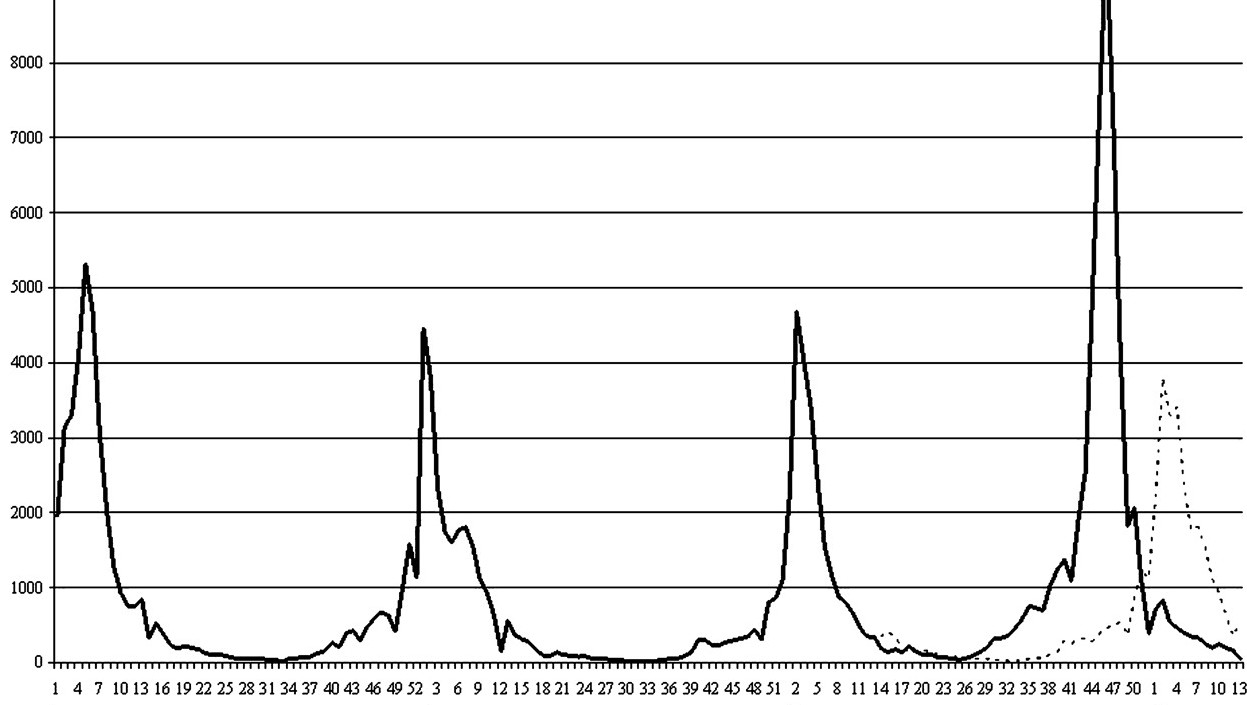
\includegraphics[height=3.0cm]{temporal_serie_cropped.jpg}
\end{center}

\end{frame}

%--------------------- slide ------------------------- %
\begin{frame}
	\frametitle{Definições}
\begin{itemize}
  \item Uma série temporal é uma sequência de $n$ números reais
				$a_1, a_2, \ldots, a_n$
  \item Eventos são variações significativas em um dado intervalo
				 de tempo
\end{itemize}

\end{frame}


%--------------------- slide ------------------------- %
\begin{frame}{Formalização}

\textbf{Entrada}: Uma série de números reais $a_1, a_2, \ldots, a_n$ (Offline)
\medskip

\textbf{Objetivo}: Responder consultas, sobre a série de entrada, definidas por 
pares $(t, d)$, onde $t$ é um \textit{inteiro} e $d$ é \textit{real} (Online)
\bigskip

\textbf{Problema 1} - Todos os Pares
\\
Encontrar todos os pares $(i, j)$, $i<j$, tais que:
			$$ j - i \le t \text{ e } a_j - a_i \ge d $$

\textbf{Problema 2} - Inícios
\\
Encontrar todos os $i$ tais que existe ao menos um $j (i < j)$, tal que:
			$$ j - i \le t \text{ e } a_j - a_i \ge d $$

\end{frame}

%--------------------- slide ------------------------- %
\begin{frame}{Exemplo - Consulta Todos os Pares}
$$<5, 2, 10, 3, 7, 6, 11>$$
\begin{center}
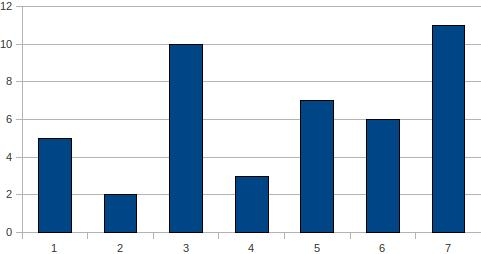
\includegraphics[height=3.0cm]{g0.jpg}
\end{center}
Consulta: $(t = 2, d = 5)$
\\
Resposta: \{\}
\end{frame}

%--------------------- slide ------------------------- %
\begin{frame}{Exemplo - Consulta Todos os Pares}
$$<5, 2, 10, 3, 7, 6, 11>$$
\begin{center}
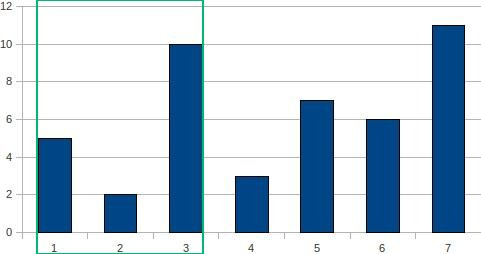
\includegraphics[height=3.0cm]{g1.jpg}
\end{center}
Consulta: $(t = 2, d = 5)$
\\
Resposta: \{$(5, 10)$\}
\end{frame}

%--------------------- slide ------------------------- %
\begin{frame}{Exemplo - Consulta Todos os Pares}
$$<5, 2, 10, 3, 7, 6, 11>$$
\begin{center}
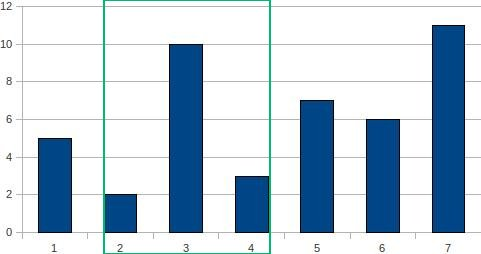
\includegraphics[height=3.0cm]{g2.jpg}
\end{center}
Consulta: $(t = 2, d = 5)$
\\
Resposta: \{$(5, 10), (2, 10)$\}
\end{frame}

%--------------------- slide ------------------------- %
\begin{frame}{Exemplo - Consulta Todos os Pares}
$$<5, 2, 10, 3, 7, 6, 11>$$
\begin{center}
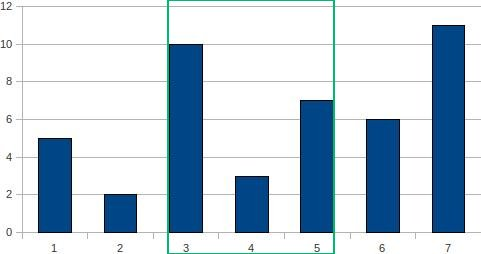
\includegraphics[height=3.0cm]{g3.jpg}
\end{center}
Consulta: $(t = 2, d = 5)$
\\
Resposta: \{$(5, 10), (2, 10)$\}
\end{frame}

%--------------------- slide ------------------------- %
\begin{frame}{Exemplo - Consulta Todos os Pares}
$$<5, 2, 10, 3, 7, 6, 11>$$
\begin{center}
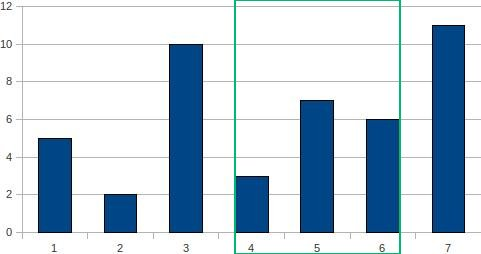
\includegraphics[height=3.0cm]{g4.jpg}
\end{center}
Consulta: $(t = 2, d = 5)$
\\
Resposta: \{$(5, 10), (2, 10)$\}
\end{frame}

%--------------------- slide ------------------------- %
\begin{frame}{Exemplo - Consulta Todos os Pares}
$$<5, 2, 10, 3, 7, 6, 11>$$
\begin{center}
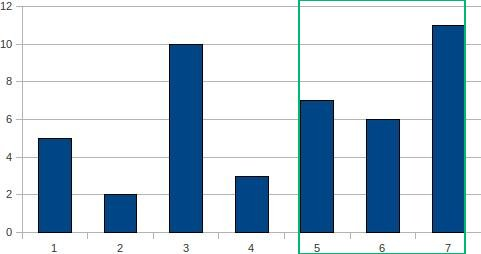
\includegraphics[height=3.0cm]{g5.jpg}
\end{center}
Consulta: $(t = 2, d = 5)$
\\
Resposta: \{$(5, 10), (2, 10)$\}
\end{frame}

%--------------------- slide ------------------------- %
\begin{frame}{Exemplo - Consulta Todos os Pares}
$$<5, 2, 10, 3, 7, 6, 11>$$
\begin{center}
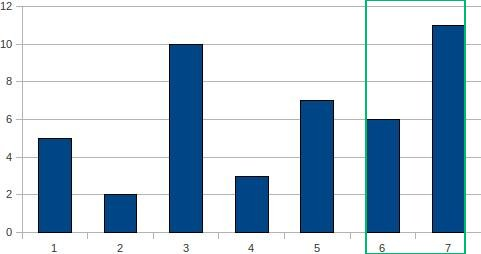
\includegraphics[height=3.0cm]{g6.jpg}
\end{center}
Consulta: $(t = 2, d = 5)$
\\
Resposta: \{$(5, 10), (2, 10),(6, 11)$\}
\end{frame}

%--------------------- slide ------------------------- %
\begin{frame}{Exemplo - Consulta Inícios}
$$<5, 2, 10, 3, 7, 6, 11>$$
\begin{center}
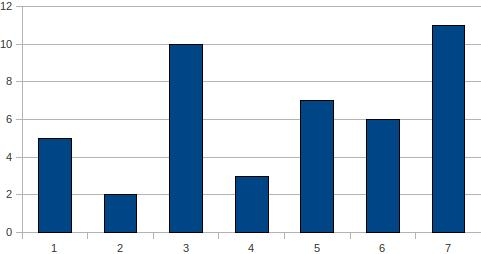
\includegraphics[height=3.0cm]{g0.jpg}
\end{center}
Consulta: $(t = 2, d = 5)$
\\
Resposta: \{$5, 2, 6$\}
\end{frame}

%--------------------- slide ------------------------- %
\begin{frame}{Exemplos}
$$<5, 2, 10, 3, 7, 6, 11>$$

\textbf{Todos os Pares}\\
Consulta: $(t = 2, d = 5)$\\
Resposta: $\{(5, 10), (2, 10), (6, 11)\}$\\
\textit{Tamanho da saída varia de $0$ até $\frac{n(n-1)}{2}$}
\bigskip

\textbf{Inícios}\\
Consulta: $(t = 2, d = 5)$\\
Resposta: $\{5, 2, 6\}$\\
\textit{Tamanho da saída varia de $0$ até $n$}
\end{frame}

%--------------------- slide ------------------------- %
\begin{frame}{Objetivos}
\begin{itemize}
\item Construir estruturas de dados que permitam responder eficientemente
			os dois tipos de consultas definidas
\item Realizar análises teóricas sobre as estruturas propostas
\item Avaliar experimentalmente as estruturas
\end{itemize}
\end{frame}

%--------------------- slide ------------------------- %
\begin{frame}{Conceitos Importantes}
\begin{itemize}
\item
Range Minimum Query (RMQ): Determinar o mínimo em um intervalo
de forma eficiente. Admite estruturas de dados com as características
abaixo:
\begin{itemize}
	\item Tempo e espaço de pré-processamento $O(n)$
	\item Consultas em $O(1)$
\end{itemize}
\end{itemize}
\begin{center}
\includegraphics[height=3.0cm]{RMQ.pdf}
\end{center}

\end{frame}

%--------------------- slide ------------------------- %
\begin{frame}{Conceitos Importantes}
\begin{itemize}
\item
Orthogonal Range Tree: Estrutura de dados que permite
reportar todos os pontos (em um plano) dentro de um 
dado retângulo de forma eficiente
\begin{itemize}
\item Tempo e espaço de pré-processamento $O(n \log n)$
\item Consultas em $O(\log n + k)$
\end{itemize}
\end{itemize}
\begin{center}
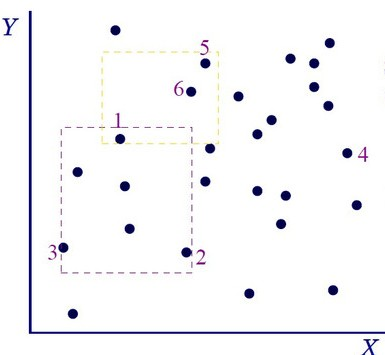
\includegraphics[height=3.0cm]{range_search.jpg}
\end{center}

\end{frame}

%--------------------- slide ------------------------- %
\begin{frame}{Solução Trivial - Todos os Pares}
\begin{itemize}
\item
Pré-processamento: Para todo par $(a_i, a_j)$, $i<j$, guardar as 
diferenças $a_j - a_i$ em um vetor ordenado
\item 
Consulta: Percorrer o vetor ordenado enquanto as diferenças
forem menores que $d$
\item
Complexidade de Tempo:
$<O(n^2 \log n), O(k)>$, onde $k$ é a quantidade de pares reportados
\item
Complexidade de Espaço: $O(n^2)$
\end{itemize}
\end{frame}

%--------------------- slide ------------------------- %
\begin{frame}{Solução Trivial - Inícios}
\begin{itemize}
\item
Pré-processamento: Criar uma estrutura de RMQ para a série
\item 
Consulta: Iterar em cada elemento da série e descobrir o maior
entre os próximos $t$ elementos
\item 
Complexidade de Tempo:
$<O(n), O(n)>$, usando uma estrutura eficiente de RMQ
\item
Complexidade de Espaço:
$O(n)$
\end{itemize}
\textit{Para $k << n$ o tempo de resposta é dominado por $n$}
\end{frame}

%--------------------- slide ------------------------- %
\begin{frame}{F-pairs}

Um \textbf{F-pair} é um par $(i, j)$, tal que:

		$$ a_i < \min\{ a_{i+1}, a_{i+2}, \ldots, a_j \}
								\text{ e }
			 a_j > \max\{ a_i, a_{i+1}, \ldots, a_{j-1} \}
		$$
Exemplo
		$$<5, 2, 10, 3, 7, 6, 11>$$
F-pairs: $\{(2, 10), (3, 7), (6, 11), (3, 11)\}$

\end{frame}


%--------------------- slide ------------------------- %
\begin{frame}{F-pairs - Propriedades}

\begin{lem}
Para toda solução $(a_i, a_j)$, temos:
\begin{enumerate}
\item $(a_i, a_j)$ é um F-pair; ou
\item $(a'_i, a_j)$ é solução, onde $a'_i$ é o início de algum F-pair; ou
\item $(a_i, a'_j)$ é solução, onde $a'_j$ é o fim de algum F-pair
\end{enumerate}
\end{lem}

\bigskip

\begin{cons}
É possível encontrar todas as soluções, para o problema \textit{Todos os Pares},
a partir dos F-pairs.
\end{cons}

\end{frame}

%--------------------- slide ------------------------- %
\begin{frame}{F-pairs - Propriedades}

Do ponto de vista da quantidade de F-pairs, toda série
pode ser mapeada em uma permutação

\begin{lem}
O valor esperado do número de F-pairs é $O(n)$,
com constante baixa e o resultado vale com
alta probabilidade
\end{lem}
\bigskip
Observação: No pior caso, a quantidade de F-pairs pode ser quadrática.

\begin{center}
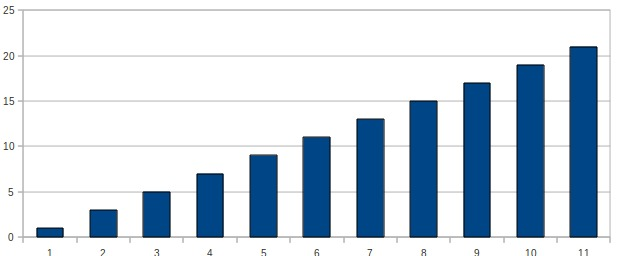
\includegraphics[height=3.0cm]{badcase.jpg}
\end{center}

\end{frame}


%--------------------- slide ------------------------- %
\begin{frame}{Abordagem Proposta - Todos os Pares}

\textbf{Abordagem}

\begin{itemize}
\item Pré-processamento: guardar todos os F-pairs em uma estrutura adequada
\item Usar os F-pairs como ponto de partida para responder as consultas
\end{itemize}

\textbf{Características da Abordagem}
\begin{itemize}
\item Tempo de resposta $O(k)$
\item Tempo de pré-processamento $O(\#\text{F-pairs})$
\item Tamanho da estrutura $O(\#\text{F-pairs})$
\end{itemize}

\end{frame}

%--------------------- slide ------------------------- %
\begin{frame}{Análise Experimental}

\begin{itemize}
\item Avaliar o tamanho das estruturas propostas em séries aleatórias
			e reais
\item Avaliar o tempo de resposta das estruturas
\item Comparar com outras estruturas 
\end{itemize}

\end{frame}

%--------------------- slide ------------------------- %
\begin{frame}{Análise Experimental - Dados}

\begin{itemize}
\item Séries geradas aleatoriamente
\begin{itemize}
\item Permutações de tamanho $1MB$, $2MB$, $3MB$, $4MB$ e $5MB$
\item Geradas de forma aleatória
\end{itemize}

\item Séries Reais
\begin{itemize}
\item $4$ séries reais advindas de dados do mercado financeiro
\item Tamanhos das séries $199258, 179443, 142941, 191672$
\end{itemize}
\end{itemize}

\end{frame}

%--------------------- slide ------------------------- %
\begin{frame}{Análise Experimental - Baselines}

\begin{itemize}
\item RMQ
\begin{itemize}
\item Tempo de resposta $O(n + k)$ para ambas as consultas
\item Tamanho $O(n)$
\end{itemize}
\end{itemize}

\end{frame}

%--------------------- slide ------------------------- %
\begin{frame}{Cronograma}
\begin{center}
\begin{tabular}{|l|l|l|l|l|l|}
\hline
\textbf{Novembro} & Desenvolver e implementar heurísticas \\
\hline
\textbf{Dezembro} & Desenvolver e implementar heurísticas \\
\hline
\textbf{Janeiro} & Experimentar com séries reais e aleatórias \\
\hline
\textbf{Fevereiro} & Escrever texto \\
\hline
\textbf{Março} & Escrever texto \\
\hline
\end{tabular}
\end{center}
\end{frame}

%--------------------- slide ------------------------- %
\begin{frame}{Referências}
\bibliographystyle{plain}
\bibliography{proposta}
\end{frame}

\end{document}
